\section{选取等高线围道}\label{sec:A}

我们召回公式 \eqref{eq:9.0.1} 中定义的函数 h:
\begin{equation}\label{eq:A.0.1}
h := \lambda + \frac{\lambda}{\lambda - 1} = -256q \prod_{n=1}^{\infty} (1 + q^n)^{24} = -256 \cdot \frac{\Delta(2\tau)}{\Delta(\tau)}, \quad q = e^{2\pi i \tau}.
\end{equation}

对于任意满足 \(\psi(0) = 0\) 的双全纯映射 \(\psi : \mathbf{D} \to \Omega \subset \mathbf{D}\), 设 \(\varphi = h(\psi(x))\). 
我们的任务是选择一个函数 \(\psi\), 使得:
\begin{itemize}
  \item[(1)] \(\psi\) 在 \(\mathbf{D}\) 内部的像排除了点 \(-1/72\) 在 h 下的所有原像, 除了唯一的实原像 \(0.0000541... \in \mathbf{R}\). （这是在实轴上唯一的原像.）
  \item[(2)] 以下量（参见等式 \eqref{eq:7.0.3}）:
  \begin{equation}\label{eq:A.0.2}
  \frac{\iint_{\mathbf{T}^2} \log |\varphi(z) - \varphi(w)| \, \mu_{\text{Haar}}(z) \mu_{\text{Haar}}(w)}{\log |256\psi'(0)| - \tau(\mathbf{b}; \mathbf{e})}
  \end{equation}
  尽可能地小, 对于某个显式常数 \(\tau(\mathbf{b}; \mathbf{e}) = \frac{16603}{3920} = \frac{27}{80} + \frac{191}{49}\).
\end{itemize}

在此处, \(\log |\psi'(0)|\) 是 \(\Omega\) 的共形半径. 
此处的难点在于我们希望 \eqref{eq:A.0.2} 的分母尽量大, 
并因此 \(\Omega \subset \mathbf{D}\) 尽量大； 
在同一时间, 当 z 在从 0 到 cusp \(e^{2\pi i\alpha}\) （其中 \(\alpha=p/q\) 且 q 是奇数）的直线上变化时, 
函数 h(z) 具有渐近增长速度:
\[ \log |h(z)| \sim \frac{1}{2\pi^2 q^2 (1 - |z|)}. \]
（所有这些都很容易从 h 是 \(\Gamma_0(2)\) 级别的模函数这一事实中得出.） 
为了选择 \(\Omega\), 最好先检验 h 的地形. 
图~\ref{fig:A.0.3} 中的阴影区域指出了满足 \(|h(z)| \geq e^{20}\) 
的 \(|z| \leq 1\) 部分, 
等等高线 \(|h(z)| \in \{1, e^4, e^8, e^{12}, e^{16}\}\), 
以及最后绕 -1/72 的原像的等高线 \(|h(z) + 1/72| = 1/200\). 
（两种等高线类型可以通过其连通分支是否含有趋近于边界的子序列来进行区分.） 

\begin{figure}[!htbp]
  \centering
  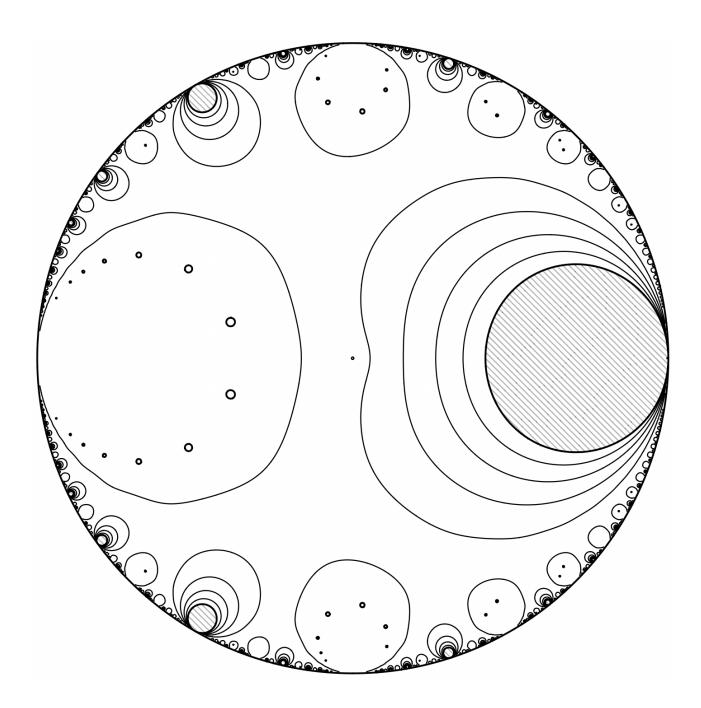
\includegraphics[width=0.55\textwidth]{assets/fig/_page_200_Picture_2.jpeg}
  \caption{阴影区域包含满足 \(|h(z)| \geq e^{20}\) 且靠近 cusp \(z = e^{2\pi i p/q}\) （其中 q 是奇数）的部分. 其他等高线为在 \(|h(z)| \in \{1, e^4, e^8, e^{12}, e^{16}\}\) 上的等高线，以及绕 -1/72 在 \(|h(z) + 1/72| = 1/200\) 的原像等高线.}\label{fig:A.0.3}
\end{figure}

构造 \(\Omega\) 的基本想法是选择一个以原点为中心、半径排除了在 \(z = \pm i\) 附近的 -1/72 
原像的圆周, 
并且然后（近似地）从 \(\Omega\) 中移除以下内容:
\begin{itemize}
  \item[(1)] 该圆周与靠近 z = 1 的 horoball 的交集.
  \item[(2)] 在靠近 z = -1 的 horoball 附近, 从该圆周到剩下的 -1/72 原像的狭缝（slits）.
\end{itemize}

Riemann 映射定理保证了对于任何此类区域 \(\Omega\) 均存在一个 \(\psi(x)\). 
然而, 我们还希望选择一个具有如下显式形式的 \(\psi(x)\), 
以便能够对 \eqref{eq:A.0.2} 进行严格的估计. 
因此在实际中, 我们选择近似该区域的简单显式函数. 
\(\Omega\) 的构造是非常定制化的, 
并且（对我们而言）完全不清楚如何在所有的 \(\Omega\) 
上最小化 \eqref{eq:A.0.2}, 
除了从我们的经验中可以说, 我们相信我们的构造与最优选择相差不远. 
我们最终选择的 \(\Omega\) 展示在图 A.4.5 中（该图还具有 \(\log |h(z)|\) 的更详细地形图）.

\subsection{关于圆弧二角形（Lunes）的准备知识}\label{sec:A.1}

设 D(c, R) 表示以 c 为中心、半径为 R 的圆盘. 
固定 c > 1, 并考虑映射:
\[ f(z,c) = z \cdot \frac{(c^2+1) + (c^2-1)z}{(c^2-1) + (c^2+1)z}. \]
该映射具有如下性质：它是一个从圆弧二角形 L(c) 
到单位圆盘的、将 z = 0 映射为 0 的共形同构, 
其中该二角形组成如下:
\[ L(c) := \mathbf{D} \setminus \mathbf{D} \cap D\left(-\frac{c^2+1}{c^2-1}, \frac{2c}{c^2-1}\right). \]
也就是单位圆盘减去两个在 \(|z| = 1\) 处以直角相交的圆盘的交集. 
（这保证了存在一个显式且初等的共形映射）. 
右侧圆周的“最内侧”点是点:
\[ -\frac{c^2+1}{c^2-1} + \frac{2c}{c^2-1} = -\frac{c-1}{c+1}. \]
在极限 \(c \to \infty\) 下, 该点趋近于 -1, 
并且区域 L(c) 趋近于整个圆盘, \(f(z)\) 趋近于 z. 
函数 f(z) 具有由下式给出的显式逆映射:
\begin{equation}\label{eq:A.1.1}
h(z,c) = \frac{z(1+c^2) - 1 - c^2 + \sqrt{(1+c^2)^2(1+z)^2 - 16c^2z}}{2(c^2 - 1)},
\end{equation}
并因此 L(c) 的共形半径为:
\begin{equation}\label{eq:A.1.2}
\frac{c^2 - 1}{c^2 + 1}.
\end{equation}

\subsection{吞噬区域（Gobbles）}\label{sec:A.2}

我们在定理 A 或 C 的证明中并未使用本节的围道, 
而是用我们在下文第 A.3 节中考虑的狭缝与圆弧二角形的组合代替了它们. 
然而, 它们在第 6.8 节定理 2.8.4 的证明中被使用了. 
此外, 我们的初版论证确实采用了它们, 
并且它们为提供在其他例子上的基准测试提供了便利的围道, 
而且也比我们稍微有些定制化的狭缝使用更灵活.

假设我们希望移除两个对称相反的圆盘, 它们并不一定具有相同的大小. 
在这种情况下没有容易表述的简单共形映射. 
然而, 作为第一步近似, 我们可能先移除一个圆盘, 
然后移除另一个. 我们定义:
\[ \operatorname{Gob}(z, e, f) := h(-h(z, f), e). \]
使用公式 \eqref{eq:A.1.1}, 这具有一个稍微有些杂乱、但完全显式的形式.

\begin{definition}\label{def:A.2.1}
在 \(\mathbf{D}\) 内部、伴随参数 \(r \in (0, 1]\), \(e \in (1, \infty]\), 以及 \(f \in (1, \infty]\) 
的吞噬区域是 \(\mathbf{D} = D(0, 1)\) 在映射:
\[ \operatorname{Gob}(r, e, f) : \mathbf{D} \to \mathbf{C}, z \mapsto r \cdot \operatorname{Gob}(z, e, f) \]
下的像. \(\triangle\)
\end{definition}

一个核心性质是, 对于极宽范围的参数, 
该吞噬区域在视觉上与 \(D(0,1)\) 中两个圆盘的补集是无法区分的, 
而在同一时间其又明显更显式、从而更容易计算. 
由显式公式, 我们很容易获得:

\begin{lemma}\label{lem:A.2.2}
以 z = 0 为中心的 \(\operatorname{Gob}(r, e, f)(\mathbf{D})\) 的共形半径等于:
\[ r \cdot \frac{(e^2-1)(f^2-1)}{(e^2+1)(f^2+1)}. \]
\end{lemma}

\subsection{狭缝（Slits）}\label{sec:A.3}

对于实数 r \(\in (0, 1)\), 从
\[ (\mathbf{D},0) \xrightarrow{\simeq} (\mathbf{D} \setminus (-1,-r],0) \]
的一个共形同构由下式定义的函数 \(\operatorname{Slit}(z, r)\) 给出:
\begin{equation}\label{eq:A.3.1}
\frac{(r+1)^2 - 2(r-1)^2 z + (r+1)^2 z^2 + (1+r)(-1+z)\sqrt{(1+r)^2 - 2(1-6r+r^2)z + (1+r)^2 z^2}}{8rz}
\end{equation}
\[ = \frac{4r}{(1+r)^2} z + \frac{8r(1-r)^2}{(1+r)^4} z^2 + \frac{4(1-r)^2 r(3-14r+3r^2)}{(1+r)^6} z^3 + \dots \]
特别地, \(\mathbf{D} \setminus (-1, -r]\) 在原点处的共形半径等于:
\begin{equation}\label{eq:A.3.2}
|\operatorname{Slit}'(0,r)| = \frac{4r}{(1+r)^2}.
\end{equation}

我们包含了对映射 \eqref{eq:A.3.1} 导出过程的一个概述. 
起步点是评述：有理变换 \(z \mapsto z/(1+z)^2\) 将我们的狭缝圆盘 \(\mathbf{D} \setminus (-1, -r]\) 
共形同构地映射为 \(\mathbf{P}^1 \setminus [-(1-r)^2/r, 1/4]\) 的倒数像. 
现在, 实轴上的线段 \([A, B] \subset \mathbf{R}\) 具有等于其长度四分之一的超限直径（外半径）. 
这已经证明了关于共形大小的公式 \eqref{eq:A.3.2}, 
因为 Riemann 映射球 \(\mathbf{P}^1 = \mathbf{C} \cup \{\infty\}\) 
中一个紧子集 K 补集在原点处的共形半径等于 K 超限直径的倒数. 
对于实际的 Riemann 映射 \eqref{eq:A.3.1}, 
我们通过观察到线段补集 \(\mathbf{P}^1 \setminus [A, B]\) 的、从 \(\infty\) 的逆 Riemann 映射由一个平方根函数给出而继续进行:
\[ \mathbf{P}^1 \setminus [A, B] \xrightarrow{\simeq} \mathbf{H}, \quad z \mapsto i\sqrt{(z-A)/(z-B)}, \quad \infty \mapsto i, \]
其逆映射为 \(z \mapsto \frac{A+Bz^2}{1+z^2}\). 
在应用 Cayley 变换 \(\mathbf{H} \xrightarrow{\simeq} \mathbf{D}\), \(z \mapsto (z-i)/(z+i)\) （其逆映射为 \(z \mapsto i(1+z)/(1-z)\)）的前提下, 
我们到达了合成的 Riemann 映射 \eqref{eq:A.3.1}.

\subsection{组合多重狭缝以及圆弧二角形}\label{sec:A.4}

假设我们希望移除四个狭缝以及一个二角形. 
在这种情况下没有容易表述的简单共形映射. 
然而, \eqref{eq:A.1.1} 以及 \eqref{eq:A.3.1} 中的两个共形映射都具有如下性质： 
它们在圆周的“大多数”点上（也就是在偏离二角形以及狭缝的点处） 
都可以被恒等映射 \(z \mapsto z\) 很好地近似. 
因此, 构造此类映射的一种非常原始的方式仅仅是依次复合这些映射. 
为此, 我们考虑以下函数:
\[ G(z) := -R \cdot h\left(-e^{2\pi i\theta_1} \cdot \operatorname{Slit}\left(e^{2\pi i\theta_2} \cdot \operatorname{Slit}\left(e^{2\pi i\theta_3} \operatorname{Slit}\left(e^{2\pi i\theta_4} \cdot \operatorname{Slit}\left(z, r_1\right), r_2\right), r_3\right), r_4\right), c\right). \]

我们固定第一个参数 R=77/100 以确保初始圆周仅包含 -1/72 在 -1 附近 horoball 中的原像, 
以及我们只需要排除 4 个此类原像. 
我们还固定了二角形参数 c=75/10, 该参数测量了我们在 z=1 附近移除的（近似）horoball. 
角度参数 \(\theta_i\) 允许我们“对齐”狭缝, 
使得它们包含了这些原像, 
并且长度参数 \(r_i\) 允许我们最小化这些狭缝的长度, 
使得它们不会越过我们希望排除的原像. 
最终的参数选择如下:
\[ R = \frac{77}{100}, \qquad c = \frac{75}{10}, \]
\[ r_1 = \frac{91}{100}, \qquad r_2 = \frac{6188}{10000}, \qquad r_3 = \frac{55515}{100000}, \qquad r_4 = \frac{772}{1000}, \]
\begin{equation}\label{eq:A.4.1}
\begin{aligned}
\theta_1 &= \frac{7977}{100000}, \qquad \theta_2 = \frac{11543}{100000}, \\
\theta_3 &= \frac{3525}{100000}, \qquad \theta_4 = -\frac{783}{10000}.
\end{aligned}
\end{equation}

这些参数选自一个临时的计算, 该计算使狭缝的端点尽可能地靠近四个参数. 
由于在数值上无法选择这些参数使得坏原像精确地位于这些狭缝上, 
我们最终定义:
\begin{equation}\label{eq:A.4.2}
\psi(z) = G\left(\frac{995}{1000} \cdot z\right).
\end{equation}

通过限制到这个开圆盘上, 我们不仅仅移除了（弯曲的）狭缝, 
还移除了开区域, 这使得证明坏原像已被排除变得非常容易. 
计算 \(\psi(z)\) 的共形半径（使用 \eqref{eq:A.1.2} 以及 \eqref{eq:A.3.2}）是非常简单的, 
它等于:
\[ |\psi'(0)| = \frac{995}{1000} \cdot R \cdot \frac{c^2 - 1}{c^2 + 1} \cdot \prod_{i=1}^{4} \frac{4r_i}{(1 + r_i)^2} \]
\begin{equation}\label{eq:A.4.3} 
= \frac{5448339453535586608000000000}{8658833407565631122430056127} = 0.6292232680... 
\end{equation}


召回 \(h: \mathbf{D} \to \mathbf{C}\) 在 \(q \in \mathbf{D}\) 下由 \(-256q \prod_{n=1}^{\infty} (1+q^n)^{24}\) 给出. 
上面选择的参数 \(r_i\) 以及 \(\theta_i\) 保证了以下结论成立:

\begin{lemma}\label{lem:A.4.4}
映射 \(\varphi := h \circ \psi : \mathbf{D} \to \mathbf{C}\) 具有唯一的 -1/72 原像.
\end{lemma}

\begin{proof}
存在一个原像满足 \(x = 0.0000541829...\). 
但人们可以通过回到 \(\mathbf{H}\) 来（以任意精度）确定其他原像, 
并且然后由 \(\Gamma_0(2)\) 的作用获得了其他的原像. 
在 \(z = \pm i\) 附近的区域（近似一 horoball）中的原像的绝对值至少为:
\[ 0.782767... > R = \frac{77}{100}. \]
最接近的其他原像位于 z = -1 附近的 horoball 附近； 
但对参数 \(r_i\) 以及 \(\theta_i\) 的精确选择确保了它们位于 \(\psi\) 像的外部, 
这可以通过简单的数值计算来予以证实.
\end{proof}

围道 \(\psi(\mathbf{T})\) 画在图~\ref{fig:A.4.5} 中. 
不对称性是由于我们使用了四个单狭缝映射的连续复合, 
而不是一次性移除所有四个狭缝.

\begin{figure}[htbp]
  \centering
  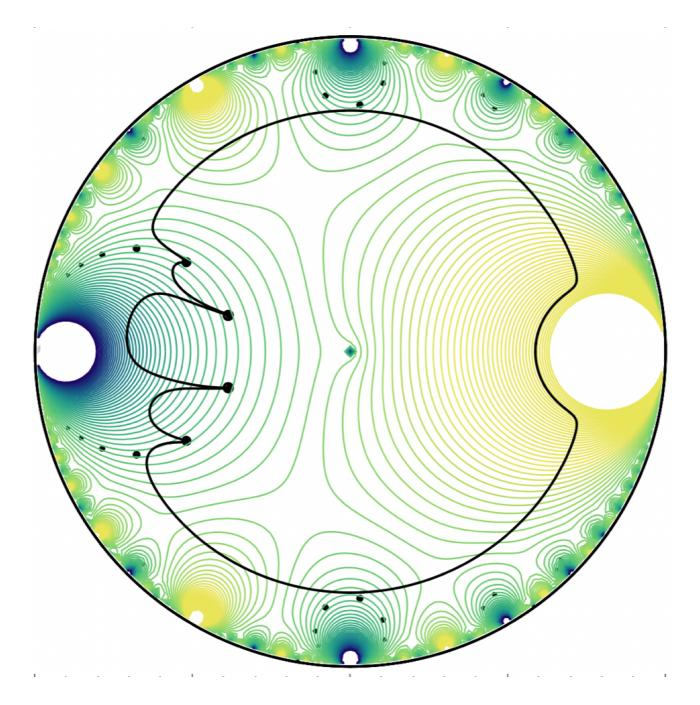
\includegraphics[width=0.45\textwidth]{assets/fig/_page_203_Figure_7.jpeg}
  \caption{\(\psi(z)\) 在 \(|z| = 1\) 处的像，以及 \(-1/72\) 在 h 下的原像，以及 \(\log |h|\) 在等差数列上的等高线. 颜色方案在黄色（正大值）与蓝色（负小值）之间转换.}\label{fig:A.4.5}
\end{figure}

\begin{remark}\label{rem:A.4.6}
我们对常数的选择仅反映了寻找一个“可行”而非最美观的例子的原理. 
这无疑存在一些改进的空间, 
但由于这不是必需的, 我们并未尝试优化这些选择——无论如何, 我们预计这两个方面的改进都将是非常温和的. \end{remark}

\subsection{针对 \texorpdfstring{$L(2, \chi_{-3})$}{L(2, \textbackslash{}chi\_\{-3\})} 问题的围道}\label{sec:A.5}

伴随我们对 \(\psi(z)\) 在等式 \eqref{eq:A.4.2} 中的特定选择, 我们现在定义:
\[ \varphi(z) = h(\psi(z)), \]
该映射在 \(\mathbf{D}\) 上是一致连续的, 
以及足够显式以至于可以进行严格的数值估计. 
我们随后最终获得了估计:
\[ \iint_{\mathbf{T}^2} \log |\varphi(z) - \varphi(w)| \, \mu_{\text{Haar}}(z) \mu_{\text{Haar}}(w) = 11.844\dots \]
以及因此, \eqref{eq:A.0.2} 被上估计为:
\begin{equation}\label{eq:A.5.1}
\frac{11.845}{\log\left(256 \cdot \frac{5448339453535586608000000000}{8658833407565631122430056127}\right) - \left(\frac{27}{80} + \frac{191}{49}\right)} = 13.9938 \dots < 14.
\end{equation}

\begin{remark}[Basic Remark A.5.2]\label{rem:A.5.2}
即使做出了我们所有的改进, 在增加积分之前, 
对于定理 A 或 C, 我们所能达到的最佳边界也都在 9 以上； 
我们现在给出其中一些数值. 
考虑定理 2.5.1 在下述情况下的基本应用. 
我们考虑在 \(\mathbf{P}^1 \setminus \{0, 1, \infty\}\) 域中的函数 \(A_i(x)\) 对于 i = 1, ..., 9. 
（在此, 前五个函数在第 10 节中显式给出, 
以及四个函数 \(A_6(x), ..., A_9(x)\) 通过那一节的变换对应于 \(B_6(z), ..., B_9(z)\). 
注意, 这些最后的四个函数只有在我们的三个周期之间存在 \(\mathbf{Q}\)-线性关系时才存在.） 
对于下式考虑定理 2.5.1:
\[ \mathbf{b} := \begin{pmatrix} 0 & 1 & 1 & 1 & 1 & 1 & 1 & 1 & 1 \\ 0 & 0 & 1 & 1 & 1 & 1 & 1 & 1 & 1 \end{pmatrix}^{\mathrm{t}} \]
并因此有 \(\sigma_1 = 0, \sigma_2 = 1\); \(\sigma_3 = \dots = \sigma_9 = 2\), 
以及:
\[ \tau(\mathbf{b}) = \frac{1 \cdot 0 + 3 \cdot 1 + (5 + 7 + 9 + 11 + 13 + 15 + 17) \cdot 2}{81} = \frac{157}{81}. \]
正如在注记 9.0.20 中解释的那样, 
如果我们使用与等式 \eqref{eq:A.4.2} 中相同的、但被拉回到 \(X(2)\) 域中的围道, 
积分项以及共形半径项都加倍了. 
等价地, 它们保持相同而 \(\tau\) 项减半了. 
因此我们在该情况下获得的对应边界为:
\begin{equation}\label{eq:A.5.3}
\frac{11.844...}{5.081...-2\cdot 157/81} = 9.833... < 10,
\end{equation}
这已经很接近但并没有形成矛盾, 因为该项并不小于 9. 
虽然这可以被稍微精细化（使用 Bost--Charles 积分以及修改围道）, 
但在不引入增加积分的前提下, 通过我们的方法似乎不太可能达到直接的矛盾； 
参见示例 7.4.9 以及 7.5.9. \end{remark}

\subsection{针对对数问题的围道}\label{sec:A.6}

我们完全可以使用与上文相同的围道来完成定理 C 的证明, 
除了伴随着一个稍微更差的常数之外. 
遵循第 14.4 节的论证, 
只要寻找满足 \(\psi\) 像排除了 z 不是太小且 h(z) 位于 \(D(0, \varepsilon^2/16)\) 内以及 h(z) 位于 \(D(0, \varepsilon^{-1})\) 
之外的区域的 \(\varepsilon\) 就已足够. 
这导致了在 \(10^7\) 以及 \(10^8\) 之间对 \(\varepsilon\) 的选择. 
然而, 在对各种不同共形映射进行优化以及使用与上文相同的映射之间的一个妥协是：直接写下简单的二角形: 
如果我们取具有共形半径为 1287/2516 以及形式为
\[ \psi(z) = -\frac{3}{4}h\left(z, \frac{23}{10}\right) \]
的二角形, 那么 \(\psi(z)\) 的像排除了所有需要的圆盘以及满足 \(|h(z)| \ge 10^6\) 以及 \(|h(z)| \le 10^{-12}2^{-4}\) 
的区域（除了在 z=0 附近的原像之外）. 
在此情况下, 我们获得了估计边界:
\begin{equation}\label{eq:A.6.1}
\iint_{\mathbf{T}^2} \log |\varphi(z) - \varphi(w)| \, \mu_{\text{Haar}}(z) \mu_{\text{Haar}}(w) \sim 9.963\dots < 10,
\end{equation}
并且我们拥有非常容易的边界:
\begin{equation}\label{eq:A.6.2}
\frac{10}{\log\left(256 \cdot \frac{1287}{2516}\right) - \frac{1032659}{242760}} = 16.103... < 17,
\end{equation}
该边界被我们在第 14.5 节中用于定理 C 的证明. 
作为比较, 我们也可以估计重排积分:
\begin{equation}\label{eq:A.6.3}
\int_0^1 2t \cdot (\log |\varphi(e^{2\pi it})|)^* dt \sim 9.972...
\end{equation}
该边界也足以证明定理 C, 此时是通过仅具有对 [0, m] 平凡划分的定理 6.0.2 获得的.

关于 \(\psi(z)\) 的像以及满足 \(|h| \ge 10^6\) 以及 \(|h| \le 10^{-12}2^{-4}\) 的区域的图像画在图~\ref{fig:A.6.4} 中.

\begin{figure}[htbp]
  \centering
  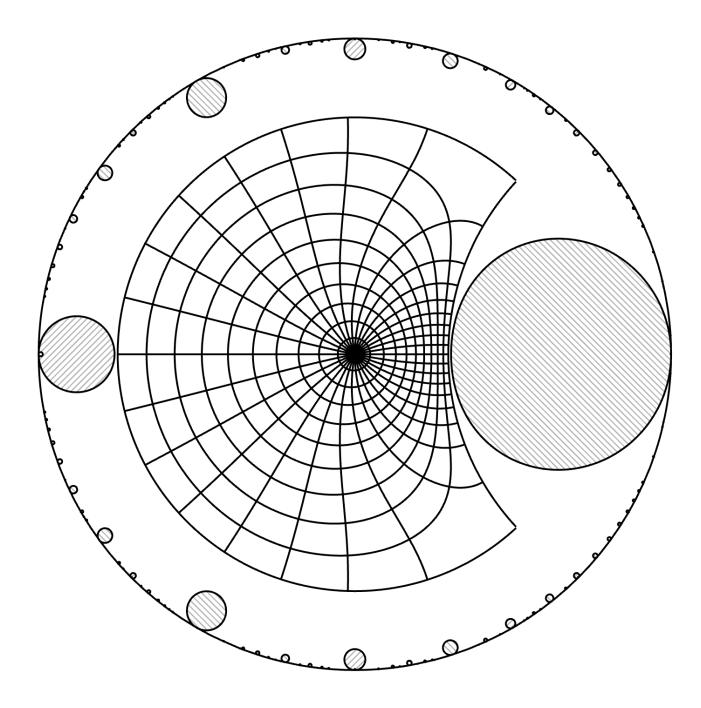
\includegraphics[width=0.45\textwidth]{assets/fig/_page_206_Figure_2.jpeg}
  \caption{\(|z| = 1\) 以及等高线在 \(\psi(z)\) 下的像，以及满足 \(|h| \geq 10^6\) 和 \(|h| < 10^{-12}2^{-4}\) 的区域（通过阴影的角度进行区分）.}\label{fig:A.6.4}
\end{figure}